
\documentclass{acm_proc_article-sp-sigmod09}

\usepackage{graphicx} 
\usepackage[english]{babel}
\usepackage{cleveref}

\begin{document}



%
% --- Author Metadata here ---
%\conferenceinfo{ACM SIGMOD}{'09 Providence, RI, USA}
%\setpagenumber{50}
%\CopyrightYear{2002} % Allows default copyright year (2002) to be over-ridden - IF NEED BE.
%\crdata{0-12345-67-8/90/01}  % Allows default copyright data (X-XXXXX-XX-X/XX/XX) to be over-ridden.
% --- End of Author Metadata ---

\title{A Sample {\ttlit ACM} SIG Proceedings Paper in LaTeX
Format\titlenote{(Produces the permission block, copyright information and page numbering). For use with ACM\_PROC\_ARTICLE-SP.CLS V2.6SP. Supported by ACM.}}
%
% You need the command \numberofauthors to handle the "boxing"
% and alignment of the authors under the title, and to add
% a section for authors number 4 through n.

\numberofauthors{2}

\author{
	Willi Menapace\\
	\texttt{203778}\\
	\texttt{willi.menapace@studenti.unitn.it}
	\and
	Luca Zanella\\
	\texttt{207520}\\
	\texttt{luca.zanella-3@studenti.unitn.it}
}

%Intro
%Data Acquisition and compression
%Data transofrmation
%Data cleaning
%Preliminary analysis
%%Introduzione di come funzionano i taxi a new york in generale eg yellow e green. Divisione della citta' in zone. Come funziona la tariffazione. Tariffe speciali per aeroporti, fare vedere mappa di dove sono gli aeroporti
%%Descrizione delle cose piu' interessanti attributo per attributo. Partiamo dal volume totale dei taxi e di come sia cambiato negli anni. Facciamo vedere i guadagni e la distribuzione negli orari e nei distretti (Facendo i punti obbligatodi dell'assignment a parte il clustering)
%%Descrizione di tutte le cose interessanti attributo per attributo
%Traffic segmentation
%%Selezione degli attributi per il clustering, selezione di k. Commenti sui cluster ottenuti. Visualizzazione grafo.
%Traffic flow analysis (Moviemnti tra le varie zone)
%Yellow vs Green
%Airport traffic analysis
%Zones classification
%
% Appendices
%
% How to run it
% Bonus section spark cluster



\maketitle
\begin{abstract}
This paper provides a sample of a \LaTeX\ document which conforms to
the formatting guidelines for ACM SIG Proceedings.
It complements the document \textit{Author's Guide to Preparing
ACM SIG Proceedings Using \LaTeX$2_\epsilon$\ and Bib\TeX}. This
source file has been written with the intention of being
compiled under \LaTeX$2_\epsilon$\ and BibTeX.

The developers have tried to include every imaginable sort
of ``bells and whistles", such as a subtitle, footnotes on
title, subtitle and authors, as well as in the text, and
every optional component (e.g. Acknowledgments, Additional
Authors, Appendices), not to mention examples of
equations, theorems, tables and figures.

To make best use of this sample document, run it through \LaTeX\
and BibTeX, and compare this source code with the printed
output produced by the dvi file.
\end{abstract}

\section{Introduction}
The NYC Taxi and Limousine Commission (TLC) has publicly made available a dataset containing data about taxi trips performed in New York from January 2009 to June 2018. This study aims at exploiting this dataset to understand how the New York taxi service works.

The report describes step by step how our analysis is performed. It starts from data acquisition, compression, transformation and cleaning and then proceeds analyzing different aspects of the data in order to provide the reader with an overview of how the taxi service in New York works.

The main technology enabling the analysis of such dataset is Apache Spark, coupled with R for data visualization.

\section{Data Acquisition and compression}

The main dataset used for the analysis is publicly available at [URL]. We download the data for the time period from January 2010 to June 2018, both for Yellow and Green taxis which consists of ~200GB of comma separated value files containing over a 1 Billion records. The schema of the dataset varies by year and taxi company for a total of 6 different schemas. The main columns available through the datasets refer to pickup and dropoff datetimes, trip distance, number of passengers, fare amount, total amount, tip amount, extras and taxes, tolls, ratecode and payment type. The most notable difference between the data is the information about pickup and dropoff locations which is expressed with latitutes and longitudes until 2016 and with numerical taxi zone identifiers for the following years.

After acquisition of the data we proceed to compress it to .tar.gz format in order to handle them more effectively. The compression is significant, with a resulting dataset size of 43GB. The gzip format however is not particularly suited for big data analysis. The parquet file format provides significant performance advantages such as columnar storage, which allows computations that only need specific columns to access them selectively, specific compression algorithms for each column with dictionary specific encodings and the possibility to decode the file even partially which is convenient in distributed environments such as Spark. The size of the dataset is slightly reduced to 39GB.

\section{Data transformation}

The parquet dataset is then transformed into a common schema format to uniform the data and ease the analysis. We decide to adopt the following schema

XXXXXXXXXXXXXXX Describe one by one

\begin{itemize}
	\item taxi\_company
	\item pickup\_datetime
	\item dropoff\_datetime
	\item pickup\_location\_id
	\item dropoff\_location\_id
	\item passenger\_count
	\item trip\_distance
	\item ratecode\_id
	\item fare\_amount
	\item tolls\_amount
	\item total\_amount
	\item mta\_tax
	\item improvement\_surcharge
	\item extra
	\item tip\_amount
	\item payment\_type
\end{itemize}

Note that the common schema codifies the pickup and dropoff locations as the ids of the zone where the pickup or the dropoff happened and not as coordinates. The main challenge for schema conversion is the transformation of dropoff and pickup locations expressed as coordinates into the respective taxi zones. The dataset is accompanied by a shapefile which specifies the geographical boundaries of each zone. Unfortunately, naive algorithms for dataset conversion directly using the shapefile are able to only convert some tens of records per second per processor which would make the conversion of 1 Billion of records unfeasible. Instead, we decide to develop a more efficient algorithm for zone association which makes use of look up tables to increase the performance of the conversion up to the thousands of records per second, allowing the complete conversion of the dataset.

\subsection{Coordinates to Zone conversion algorithm}
XXXXX

DIre che la dimensione e' 24GB.

\section{Data cleaning}

An analysis of the dataset in the common format highlights data quality problems in some of its entries. To increase the quality of the analysis we decide to perform some data cleaning on the dataset.
Null entries are a minority of the dataset, so we decide to drop every entry in the dataset with a null attribute. Every categorical feature is then enforced to assume a value in its set of legal values. In particular, location ids are enforced to be valid ids and each entry for which our coordinate conversion algorithm was not able to identify a correspondent taxi zone is dropped. We then plot the distribution of the values of each numerical feature and conservatively identify a point in its tail after which all entries are dropped, for example tolls amounts greater than 120\$ are discarded because very irrealistic according to the distribution of the tolls and probably symptom of poor data quality. We also conservatively drop entries for which the duration is greater than 24 hours or for which the year is not in the range from 2010 to 2018.

The resulting dataset contains 1.07 Billion entries versus the original 1.38 Billion entries and the size of the dataset reduced to 20GB.

%1376582531 initial entries
%1077952992 final entries


\section{Preliminary analysis}
The first phase of the analysis is the study of the domain. The New York taxi service is operated by private individuals owning taxi licenses. Two kind of taxi cabs are present, each one with specific characteristics and limitations: yellow cabs, also called medallion taxis, and green cabs, also called boro taxis. The city of New York is divided in five different districts called boroughs, shown in \cref{fig:boroughsMap}: Manhattan, Bronx, Brooklyn, Queens and Staten Island and each one is further divided into taxi zones. Both yellow and green taxis share the same fare system, but, while yellow cabs are allowed to pickup passengers anywhere in the five boroughs, green cabs are not allowed to pick up passengers in South Manhattan, LaGuardia Airport and JFK Airport, the most profitable zones for yellow taxis, but are allowed to drop the passengers anywhere. The reasons for the limitations of green taxis are two. The first is that before the introduction of green taxis, finding a cab in the boroughs outside Manhattan was challenging because yellow taxis prefer to stay in the more profitable Manhattan zone, so this limitation favors the distribution of taxis in the outer zones. The second reason is that the introduction of new licenses for green taxis was seen as a menace from the yellow cab business which strongly opposed to their introduction and obtained that green taxis would not be allowed to pick up passengers at the lucrative LaGuardia and JFK airport zones unless previously arranged by passengers with the driver.

\begin{figure}
	\centering
	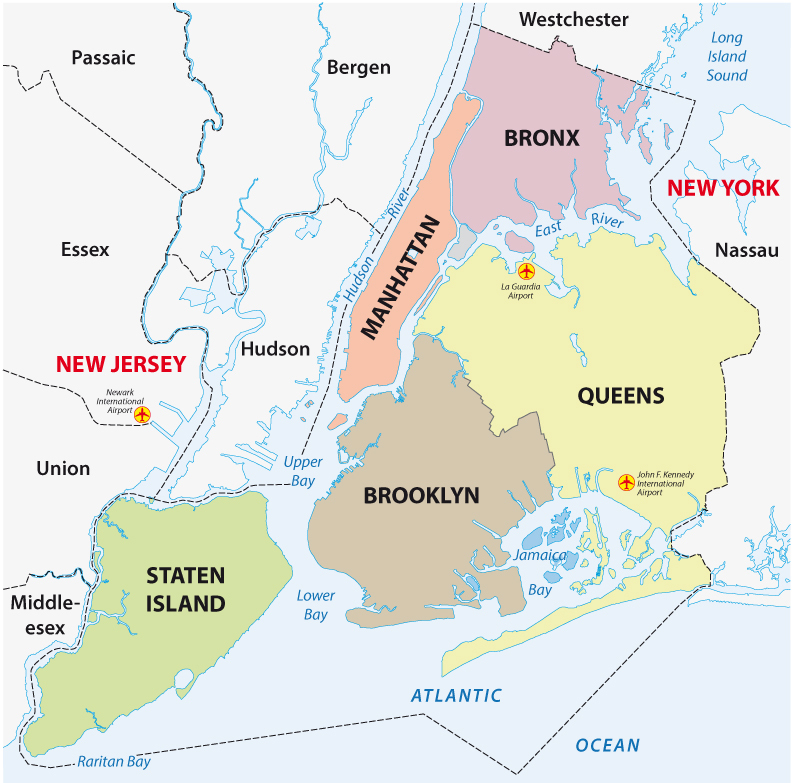
\includegraphics{resources/boroughsMap.jpg}
	\caption{The five boroughs of New York. Note the position of the three airports: LaGuardia, JFK and Newark.}
	\label{fig:boroughsMap}
\end{figure}

The fare system is shared by both yellow and green cabs. The amount starts from a base of 2.50\$ and increases as a function of time when moving slowly and as a function of distance when moving faster. Some extras may be added based on the hour of the day as well as various taxes. The passenger is also requested to pay for any incurred toll and is requested to tip the driver with a variable amount that ranges around 20\% of the total. Fares between any zone of Manhattan and LaGuardia airport have a special flat rate of 52\$ plus extras. Newark airport also havs a special rate which adds a 17.50\$ surcharge.

The analysis starts with a high level, exploration of the data.  XXXXXXXXXXXXXXXXXX TABLE WITH MEAN AND VARIANCE OF EACH XXXXXXXXXXXXXX As shown in XXXXXXXXXXXXX the number of total trips performed in the years grows slightly until 2015 and decreases in the following years. Note immediately that 2010 and 2016 are anomalous years due to data quality problems that caused the removal of entire months of entries for those year. Looking at the profits, calculated based on the total amount we can see an increasing trend in the years until 2015, after which there is a drop in the profits because of the reduced number of trips performed by the taxis. The growth of the profits, despite the only slight increase of the number of trips is given by a higher cost per trip in the years, as shown in XXXXXXXXXXXXX. The decline of the number of taxi trips started in 2015 can be explained by the growth in popularity of ride hailing services such as Uber which are becoming widespread in the city.

The study continues with the analysis of pickups and dropoffs. As depicted in XXXXX we can see that the periods of major activity for pickups are 8-16 and 20-24. The dropoffs follow the same pattern. Interestingly, by looking at the variation of the average speed through the day as shown in XXXXXXXXX we note that there is an inverse relationship between number of pickups and average speed, suggesting that in the highlighted time frames the city is subject to higher traffic congestions.
The most active pickup zones, as we can see from XXXXXXX are Manhattan, the part of Brooklyn closer to Manhattan, LaGuardia and JFK airports. The dropoff zones closely follow the pattern of the pickup zones, but are slightly more evenly distributed across all zones. It must be noted however that the majority of the activity is concentrates in the most profitable Manhattan and airport sectors. XXXXX shows an alternative visualization of pickup locations that highlights better the concentration of pickup activity in the zones noted above.

It is also interesting to notice how total amounts relate to the pickup location. As depicted in XXXXXX it can be noted that there is an inverse relationship between average total amount and zone distance from Manhattan. This is an expected outcome of the fact that Manhattan is one of the favourite dropoff locations, so on average the furthest zones from it are the most expensive. XXXXXX shows average trip distance by pickup location. Here we can note the direct correlation with the average total amount of the preceding picture. The average total amount also varies during the day, as depicted in XXXXXXX. Two different peak periods are identified around 5 and 16. The discontinuity at 16 is caused by the introduction of a 1\$ extra from 16 to 20 as a standard component of the fare amount, while the peak at 5 is caused by a sharp increase of the average trip distance from 2.92 to 4.61 miles due to an increased proportion of people going to the airport early in the morning with respect to the normal traffic.
We also noted a general increase of the total amount during the years as noted in XXXXXX which is a consequence of (la base fare amount da 2\$ a 2,50, generale aumento leggero dei tolls, comunque leggero aumento delle fare, introduzione improvement surcharge, extra che non erano registrati, percentuale di persone che paga con carta di credito ) XXXXXXXXXXXX taxes XXXXXXXXXXXXXXXX
The overall distribution of fare amounts is shown in XXXXXX. Note the sharp discontinuity at 52\$. This represents the special fare rate of trips linking Manhattan to the JFK airport.

A consistent part of the total amount is given by tips....

Tips

Distanza e' una trimodale.
Tolls




\section{The {\secit Body} of The Paper}
Typically, the body of a paper is organized
into a hierarchical structure, with numbered or unnumbered
headings for sections, subsections, sub-subsections, and even


\section{Conclusions}
This paragraph will end the body of this sample document.
Remember that you might still have Acknowledgments or
Appendices; brief samples of these
follow.  There is still the Bibliography to deal with; and
we will make a disclaimer about that here: with the exception
of the reference to the \LaTeX\ book, the citations in
this paper are to articles which have nothing to
do with the present subject and are used as
examples only.


%
% The following two commands are all you need in the
% initial runs of your .tex file to
% produce the bibliography for the citations in your paper.
\bibliographystyle{abbrv}
\bibliography{main}


\balancecolumns
\appendix
%Appendix A
\section{Headings in Appendices}
First appendix
\end{document}
